\section{Problem von Okamura und Seymour}

\texttt{KANTENDISJUNKTES WEGPACKUNGSPROBLEM}
\begin{itemize}
	\item \textbf{Gegeben}: Graph $G=(V,E)$ und Paare von Knoten $\{s_1,t_1\},\ldots,\{s_k,t_k\}, s_i,t_i\in V$
	\item \textbf{Gesucht}: Paarweise kantendisjunkter $s_i$-$t_i$-Wege $p_i$ in $G, 1 \leq i \leq k$
\end{itemize}
$s_i,t_i$ werden \textbf{Terminale} genannt, die Mengen $\{s_i,t_i\}$ heißen \textbf{Netze}.

Problem ist $\mathcal{NP}$-vollständig, auch falls $G$ planar ist. Wir werden das Problem deshalb später einschränken.\\

\textbf{Definition}: Sei $G=(V,E), X\subseteq V$. Dann heißt
$$\text{cap}(X)\coloneqq |\{uv\in E\mid u\in X, v\in V\setminus X\}|$$
die \textbf{Kapazität} von $X$. Zu $G$ sei $D=\{\{s_i,t_i\}\mid s_i,t_i\in V,1\leq i\leq k\}$ gegeben. Dann heißt
$$\text{dens}(X)\coloneqq|\{\{s_i,t_i\}\in D\mid |\{s_i,t_i\}\cap X|=1\}|$$
die \textbf{Dichte} von $X$. Weiterhin bezeichnet
$$\text{fcap}(X)\coloneqq \text{cap}(X)-\text{dens}(X)$$
die \textbf{freie Kapazität} von $X$. $X$ heißt \textbf{saturiert}, falls $\text{fcap}(X)=0$ und \textbf{übersaturiert}, falls $\text{fcap}(X)<0$.
\begin{center}
	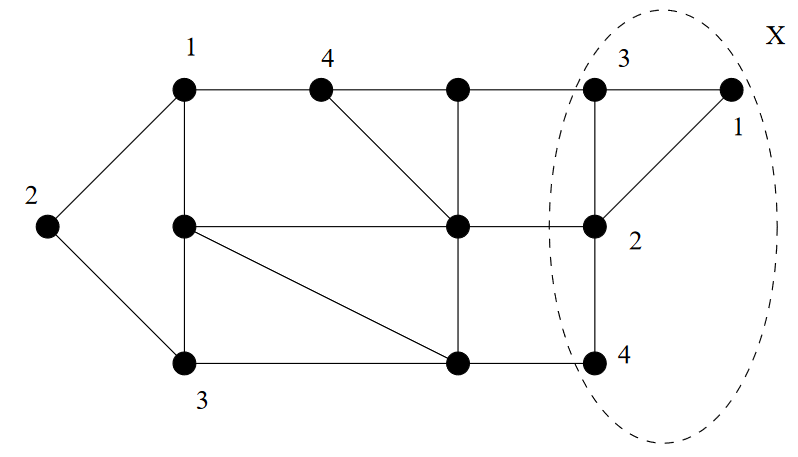
\includegraphics[width=0.4\textwidth]{images/s1.png}
\end{center}
\pagebreak
\textbf{Definition}:
\begin{itemize}
	\item \textbf{Kapazitätsbedingung}: $\text{fcap}(X)\geq 0$ für alle $X\subseteq V$. Jedes lösbare \texttt{KANTENDISJUNKTE WEGPACKUNGSPROBLEM} erfüllt die Bedingung, aber nicht jedes Problem, das die Bedingung erfüllt, ist lösbar.
	\begin{center}
		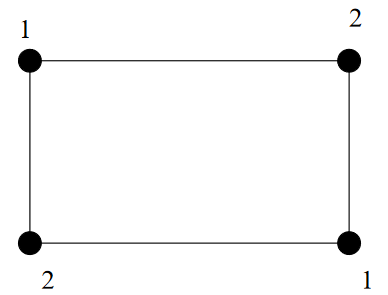
\includegraphics[width=0.2\textwidth]{images/s2.png}
	\end{center}
	$\text{cap}(X)\geq 2$ für alle $X\neq \emptyset$ und $\text{dens}(X)\leq 2$, aber nicht lösbar
	\item \textbf{Geradheitsbedingung}: $\text{fcap}(X)$ ist gerade für alle $X\subseteq V$
\end{itemize}
\bigskip
\textbf{Lemma}: Sei $G=(V,E)$ und $D=\{\{s_i,t_i\}\mid s_i,t_i\in V,1\leq i\leq k\}$. Es gilt $\text{fcap}(X)$ gerade für alle $X\subseteq V$ $\iff \text{fcap}(v)\coloneqq\text{fcap}(\{v\})$ gerade für alle $v\in V$

\textit{Beweis}:
\begin{itemize}
	\item \enquote{$\Rightarrow$}: Trivial.
	\item \enquote{$\Leftarrow$}: Sei $\text{fcap}(v)$ gerade für alle $v\in V$. Für $X\subseteq V$ ist
	\begin{itemize}
		\item $\text{cap}(X)=\sum\limits_{v\in X} \text{cap}(v)-2\cdot |\{uv\in E\mid u,v\in X\}|$
		\item $\text{dens}(X)=\sum\limits_{v\in X}\text{dens}(v)-2\cdot |\{\{s_i,t_i\}\in D\mid s_i,t_i\in X\}|$
	\end{itemize}
	Dann ist:
	$$
	\begin{aligned}
		\operatorname{fcap}(X)= & \sum_{v \in X} \operatorname{cap}(v)-\sum_{v \in X} \operatorname{dens}(v)-2 \cdot|\{uv \in E: u, v \in X\}| \\
		& +2\cdot\left|\left\{\left\{s_{i}, t_{i}\right\} \in D: s_{i}, t_{i} \in X\right\}\right| \\
		= & \sum_{v \in X} \operatorname{fcap}(v)-2 \cdot(|\{uv \in E: u, v \in X\}| \\
		& \left.+2\cdot\left|\left\{\left\{s_{i}, t_{i}\right\} \in D: s_{i}, t_{i} \in X\right\}\right|\right)
	\end{aligned}
	$$
	Also ist $\text{fcap}(X)$ gerade, falls alle $\text{fcap}(v)$ gerade sind.
\end{itemize}
\bigskip
\texttt{OKAMURA \& SEYMOUR-PROBLEM}:
\begin{itemize}
	\item \textbf{Gegeben}: Graph $G=(V,E)$ und Paare von Knoten $\{s_1,t_1\},\ldots,\{s_k,t_k\}, s_i,t_i\in V$, wobei alle $s_i,t_i$ auf dem Rand der selben Facette, o.B.d.A der äußeren, liegen.  Außerdem sei die Geradheitsbedingung erfüllt.
	\item \textbf{Gesucht}: Paarweise kantendisjunkter $s_i$-$t_i$-Wege $p_i$ in $G, 1 \leq i \leq k$
\end{itemize}
\pagebreak
\textbf{Satz}: Gegeben sei ein planar eingebetteter Graph $G = (V, E)$ und $D=\{\{s_1,t_1\},\ldots,\{s_k,t_k\}\}$, wobei $s_1,\ldots,s_k,t_1,\ldots,t_k$ auf dem Rand der äußeren Facette von $G$ liegen. Die Kapazitätsbedingung und die Geradheitsbedingung seien erfüllt. Dann existieren paarweise kantendisjunkte $s_i$-$t_i$-Wege in $G$. \qquad \textit{ohne Beweis}.\\

\textbf{Definition}: $G = (V, E)$ mit $D=\{\{s_1,t_1\},\ldots,\{s_k,t_k\}\}$ hat \textbf{Klammerstruktur}, falls $G + D$ so planar eingebettet werden kann, dass die Kanten aus $D$ kreuzungsfrei in die äußere Facette der entsprechenden Einbettung von $G$ eingebettet sind\\

\textbf{Linearzeitalgorithmus für das \texttt{OKAMURA \& SEYMOUR-PROBLEM}}:

\textbf{Schritt 1}: Konstruiere aus $G=(V,E)$ mit $D=\{\{s_1,t_1\},\ldots,\{s_k,t_k\}\}$ ein Problem bestehend aus $G=(V,E)$ mit $D'=\{\{s_1',t_1'\},\ldots,\{s_k',t_k'\}\}$ so, dass $\{s_1,\ldots,s_k,t_1,\ldots,t_k\}=\{s_1',\ldots,s_k',t_1',\ldots,t_k'\}$ und die $\{s_1',t_1'\},\ldots,\{s_k',t_k'\}$ Klammerstruktur haben
\begin{itemize}
	\item Klammerstruktur leicht in $\mathcal{O}(n)$ konstruiert werden
	\item Wähle beliebiges Terminal als Startterminal $s$ und gehe  im Gegenuhrzeigersinn um die äußere Facette
	\item Dem jeweils ersten Terminal eines $\{s_i,t_i\}$ ordne eine öffnende Klammer zu und dem jeweils zweiten eine schließende
	\begin{center}
		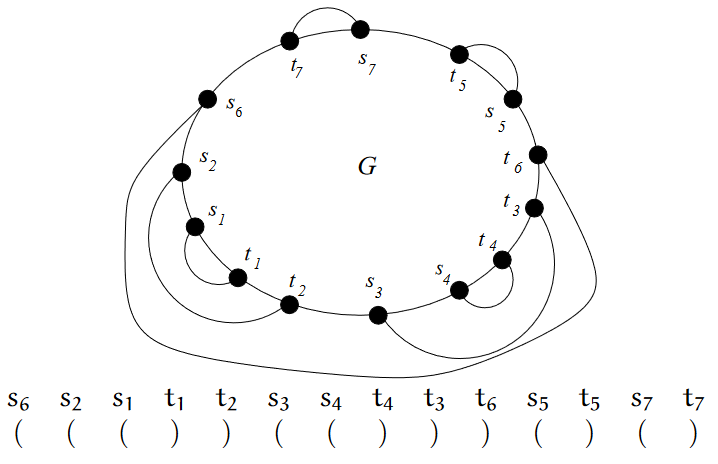
\includegraphics[width=0.5\textwidth]{images/s3.png}
	\end{center}
\end{itemize}

\textbf{Schritt 2}: Berechne in $\mathcal{O}(n)$ kantendisjunkte $s_i'$-$t_i'$-Wege $q_1,\ldots,q_k$ mittels Right-First-Tiefensuche und eine Orientierung der entsprechenden Wege von $s_i'$ nach $t_i'$
\begin{itemize}
	\item Die $s_i',t_i'$ seien, beginnend beim Startterminal $s$ im Gegenuhrzeigersinn so angeordnet,
	dass jeweils $s_i'$ vor $t_i'$ und $t_i'$ vor $t_{i+1}'$
	\item Füge zusätzlich aus technischen Gründen (s. Algorithmus S. 7) Dummy-Kanten hinzu
	\begin{center}
		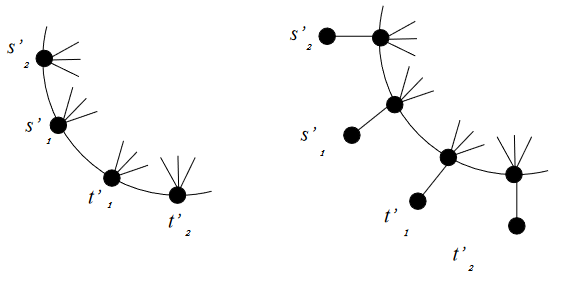
\includegraphics[width=0.5\textwidth]{images/s4.png}
	\end{center}
	\item Wegen der Geradheitsbedingung endet jeder Durchlauf der Right-First-Tiefensuche bei einem Terminalknoten
\end{itemize}

\textbf{Beobachtung}: Wegen der Right-First-Auswahlregel können an einem Knoten $v$ folgende Reihenfolgen von Kanten nicht vorkommen:
\begin{center}
	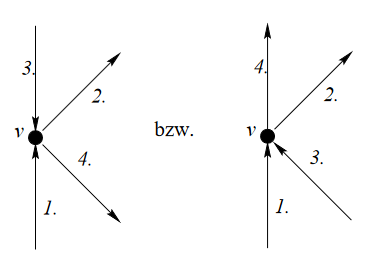
\includegraphics[width=0.25\textwidth]{images/s5.png}
\end{center}
Daher gilt für die Wege $q_i$:
\begin{itemize}
	\item Keine zwei Wege $q_i$ und $q_j$ kreuzen sich
	\item Kein Weg $q_i$ kreuzt sich selbst
\end{itemize}

Sei $\overrightarrow{G}=(\overrightarrow{V},\overrightarrow{E}), \overrightarrow{V}\subseteq V$ der Graph, der durch die von $q_1,\ldots,q_k$ belegten Kanten zusammen mit der Orientierung induziert wird.

\textbf{Korollar}: $\overrightarrow{G}=(\overrightarrow{V},\overrightarrow{E})$ enthält keinen Rechtskreis.

\textit{Beweis}:
\begin{itemize}
	\item Wenn $\overrightarrow{C}$ Kanten eines Rechtskreises in $\overrightarrow{G}$ sind, so gehören nicht alle Kanten aus $\overrightarrow{C}$ zum selben Weg $q_i$, da sich Wege nicht kreuzen
	\item Seien $q_i,q_j$, Wege, die Kanten aus $\overrightarrow{C}$ besetzen. Da $q_i$ und $q_j$ sich nicht kreuzen müssen die Terminale $s_i',t_i'$ und $s_j',t_j'$ in der Reihenfolge $s_i',t_j',s_j',t_i'$ im Gegenuhrzeigersinn auf der äußeren Facette liegen.
	\item Widerspruch zur Anordnung der Terminale.
\end{itemize}

\textbf{Korrektheit von Schritt 2}: Die Right-First-Tiefensuche berechnet für einen Graphen mit Struktur nach Schritt 1 kantendisjunkte $s_i'$-$t_i'$-Wege $q_1,\ldots,q_k$.
\begin{itemize}
	\item Betrachte eine beliebige kreuzungsfreie Lösung $q_1',\ldots,q_k'$. Eine solche Lösung existiert immer
	\pagebreak
	
	\item Wenn $q_1',\ldots,q_k'$ kreuzungsfrei ist, so gilt für jedes $q_i'$ , dass es vollständig zur linken Seite aller $q_1',\ldots,q_{i-1}'$ gehört
	\item Für jedes $q_i$ gilt, da es mittels Right-First-Auswahlregel und entsprechend der Klammerstruktur von $D'$ bestimmt wurde, dass die linke Seite von $q_i'$ ganz enthalten ist in der linken Seite von $q_i$
	\item Daraus folgt, dass $q_i$ die Terminale $s_i'$ und $t_i'$ verbindet
\end{itemize}

\textbf{Laufzeit von Schritt 2}: Amortisiert in $\mathcal{O}(n)$ realisierbar, da die rechteste freie Kante bzgl. der führenden Kante immer die nächste Kante nach der führenden Kante in der Adjazenzliste ist, und damit in konstanter Zeit gefunden werden kann

\textbf{Schritt 3}: Berechne in $\mathcal{O}(n)$ kantendisjunkte $s_i$-$t_i$-Wege $p_1,\ldots,p_k$ in $\overrightarrow{G}$ mittels gerichteter Right-First-Tiefensuche, und zwar der Reihe nach entsprechend der Reihenfolge der $t_i'$.

\textbf{Korrektheit von Schritt 3}:
\begin{itemize}
	\item Konstruiere Weg $p$ mit der Eigenschaft:
	\begin{enumerate}
		\item Falls $p_i$ korrekt $s_i$ mit $t_i$ verbindet, so induz. $p$ einen saturierten Schnitt in $G$
		\item Falls $p_i$ Terminal $s_i$ nicht mit $t_i$ verbindet, aber jedes $p_j, 1\leq j<i$ korrekt $s_j$ mit $t_j$ verbindet, so induziert $p$ einen übersaturierten Schnitt in $G$
	\end{enumerate}
	\item Mit 2. ist die Kapazitätsbedingung und damit eine notwendige Bedingung für Lösbarkeit, verletzt, also existiert in dem Fall sowieso keine Lösung
	\item Berechne $p$, der einen Schnitt mit den gewünschten Eigenschaften induziert, mit einer Left-First-Tiefensuche rückwärts vom Endknoten $t$ des $i$-ten Weges $p_i$. Das ist offensichtlich in $\mathcal{O}(n)$ möglich.
\end{itemize}

\textbf{Lemma}: Weg $p$, der wie oben berechnet wird, enthält keine Kreuzung. Insbesondere sind seine linke und rechte Seite wohldefiniert.

\textit{Beweis}: 
\begin{itemize}
	\item Angenommen $p$ würde sich selbst in einem Knoten $v$ kreuzen
	\item Da $\overrightarrow{G}$ keinen Rechtskreis enthält, gibt es in $v$ einen einfachen Linkskreis, wobei die entsprechenden Kanten von $p$, die zu $v$ inzident sind, folgende Konstellation bilden:
	\begin{center}
		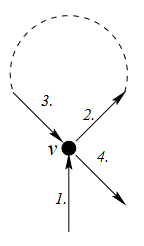
\includegraphics[width=0.1\textwidth]{images/s6.png}
	\end{center}
    \item Widerspruch zur Right-First-Tiefensuche aus Schritt 2.
\end{itemize}

\textbf{Lemma}: Sei $A$ die Menge der Kanten $uv$ aus $G$ mit $u$ auf $p$ und $v$ rechts von $p$.
Jede Kante $uv\in A$ mit $u$ auf $p$ gehört zu $\overrightarrow{G}$, und zwar in der Orientierung $(u,v)$
genau dann, wenn sie von einem der $p_j, 1\leq j<i$, besetzt ist.

\textit{Beweis}: 
\begin{itemize}
	\item \enquote{$\Leftarrow$}: Sei $uv\in A$ mit $u$ auf $p$. Falls $uv$ von einem der $p_j, 1\leq j<i$ besetzt ist, so ist deren Orientierung $(u,v)$ in $\overrightarrow{G}$, nach Konstruktion von $p$
	\item \enquote{$\Rightarrow$}: 
	
	\textbf{Fall 1}: Angenommen $uv\in A$ mit $u$ auf $p$ habe Orientierung $(u,v)$ in $\overrightarrow{G}$ und sei nicht durch eines der $p_i$ besetzt
	\begin{itemize}
		\item Betrachte die zu $p$ gehörenden Kanten $(x, u), (u, y)$ inzident zu $p$, für die $uv$ rechts von $(x, u)$ und $(u, y)$ liegt
		\item Kante, die bei der Berechnung der $p_1,\ldots,p_i$ unmittelbar vor $(u, y)$ gewählt wurde, ist dann $(x, u)$ oder liegt links von $(x, u)$ und $(u, y)$ wegen der Konstruktion von $p$
		\item Dann ist aber die Wahl von $(u, y)$ ein Widerspruch zur Right-First-Auswahlregel
		\begin{center}
			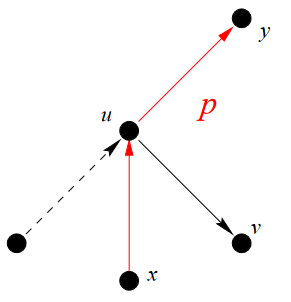
\includegraphics[width=0.2\textwidth]{images/s7.png}
		\end{center}
	\end{itemize}

	\textbf{Fall 2}: Kante $uv\in A$ mit $u$ auf $p$ gehört nicht zu $\overrightarrow{G}$
	\begin{itemize}
		\item Wegen der Right-First Auswahlregel können die Kanten $(x,u),(u,y)$ von $p$, für die $uv$ rechts liegt, nicht beide zu dem selben Weg $q_i'$ aus $\overrightarrow{G}$ gehören
		\item Gehöre $(x,u)$ zu $q_j'$ und $(u,y)$ zu $q_l'$
		\item Dann liegt Vorgängerkante von $(u,y)$ auf $q_l'$ rechts von $uv$ und $(u,y)$ und kann daher von keinem der $p_1,\ldots,p_i$ besetzt sein, da sonst $p$ wegen Left-First-Tiefensuche über $q_l'$ verlaufen würde
		\item Dann muss es eine weitere Kante $(z, u)$ in $\overrightarrow{G}$ geben, die von einem der $p_1,\ldots,p_i$ besetzt ist und links von $(x,u)$ und $(u,y)$ liegt, und eine weitere Kante $(u,w)$, die Nachfolgerkante von $(z, u)$ auf dem entsprechenden Weg $q_r'$ in $\overrightarrow{G}$ ist, und auch links von $(x,u)$ und $(u,y)$ liegt
		\item Dann liegt aber die Kante $uv$ rechts von $q_r'$ im Widerspruch zur Right-First-Auswahlregel
		\begin{center}
			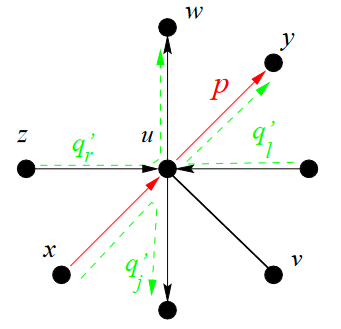
\includegraphics[width=0.2\textwidth]{images/s8.png}
		\end{center}
	\end{itemize}
\end{itemize}

\textbf{Lemma}: Sei $X\subseteq V$ Menge der Knoten rechts von $p$. Falls $p_i$ ein $s_i$-$t_i$-Weg ist, ist $X$
saturiert, ansonsten ist $X$ übersaturiert

\textit{Beweis}: Alle Kanten $\{u, v\}$ mit $u$ auf $p$ und $v \in X$ gehören entweder zu einem Weg $p_{j}$, $1 \leq j<i$, mit $s_{j} \in V \backslash X$ und $t_{j} \in X$, oder zu einem Weg $q_{j}^{\prime}$, mit $s_{j}^{\prime} \in X$ und $t_{j}^{\prime} \in V \backslash X$. Wenn $p_{i}$ ein $s_{i}$-$t_{i}$-Weg ist, dann ist damit
$$
\begin{aligned}
	\operatorname{cap}(X)= & \left|\left\{\left\{s_{j}, t_{j}\right\}: s_{j} \in V \backslash X, t_{j} \in X, 1 \leq j \leq i\right\}\right| \\
	& +\mid\left\{\left\{s_{j}^{\prime}, t_{j}^{\prime}\right\}: s_{j}^{\prime} \in X \text { und } t_{j}^{\prime} \in V \backslash X,\left\{s_{j}^{\prime}, t_{j}^{\prime}\right\} \notin\left\{\left\{s_{1}, t_{1}\right\}, \ldots,\left\{s_{i}, t_{i}\right\}\right\}\right\} \mid \\
	= & \operatorname{dens}(X) .
\end{aligned}
$$
Wenn $p_{i}$ kein $s_{i}$-$t_{i}$-Weg ist, so verbindet $p_{i}$ das Terminal $s_{i}$ mit einem Terminal $t \in$ $\left\{t_{j} ; i<j \leq k\right\}$. Da $s_{i} \in V \backslash X$ und $t_{i} \in X$ ist, dann gilt
$$
\operatorname{cap}(X) \leq \operatorname{dens}(X)-1
$$
\begin{center}
	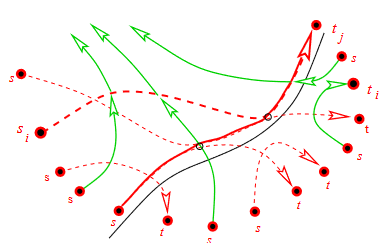
\includegraphics[width=0.4\textwidth]{images/s9.png}
\end{center}

\textbf{Laufzeit von Schritt 3}: Mit Union-Find kann die Right-First-Tiefensuche zu Schritt 3 in $\mathcal{O}(n)$ realisiert werden

V\textit{isualisierung des Algorithmus ab S.13 im Skript}